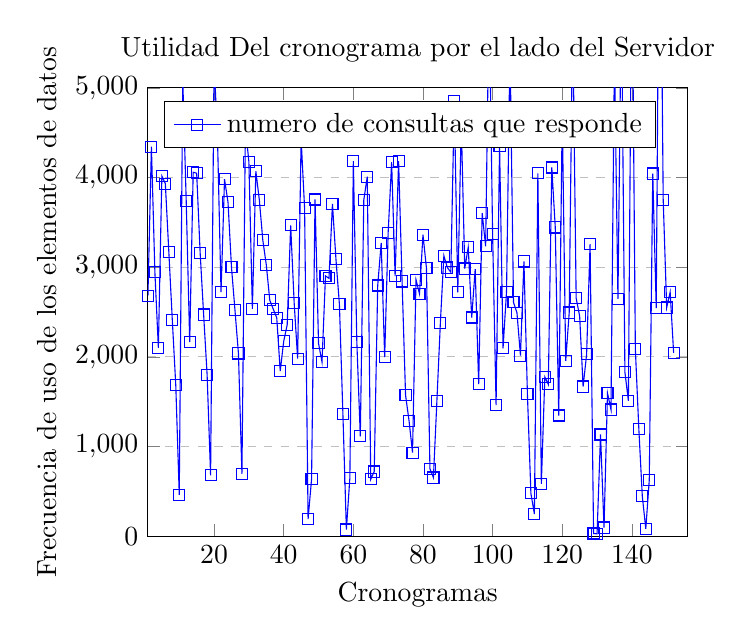
\begin{tikzpicture}
\begin{axis}[
    title={Utilidad Del cronograma por el lado del Servidor},
    xlabel={Cronogramas},
    ylabel={Frecuencia de uso de los elementos de datos},
    xmin=1, xmax=156,
    ymin=0, ymax=5000,
    xtick={},
    ytick={},
    legend pos=north west,
    ymajorgrids=true,
    grid style=dashed,
]

\addplot[
    color=blue,
    mark=square,
    ]
    coordinates {
%UTILIDAD TOTAL
%(cronograma, numero cues que usan al cronograma)
(1,2683)
(2,4344)
(3,2944)
(4,2101)
(5,4017)
(6,3932)
(7,3174)
(8,2413)
(9,1682)
(10,462)
(11,5100)
(12,3734)
(13,2165)
(14,4059)
(15,4048)
(16,3159)
(17,2472)
(18,1801)
(19,678)
(20,5303)
(21,4414)
(22,2722)
(23,3982)
(24,3725)
(25,2999)
(26,2521)
(27,2038)
(28,694)
(29,4562)
(30,4175)
(31,2536)
(32,4070)
(33,3750)
(34,3300)
(35,3026)
(36,2631)
(37,2533)
(38,2436)
(39,1842)
(40,2174)
(41,2357)
(42,3467)
(43,2605)
(44,1980)
(45,4431)
(46,3657)
(47,191)
(48,635)
(49,3755)
(50,2151)
(51,1943)
(52,2903)
(53,2875)
(54,3706)
(55,3092)
(56,2585)
(57,1367)
(58,74)
(59,649)
(60,4184)
(61,2170)
(62,1113)
(63,3749)
(64,4009)
(65,635)
(66,721)
(67,2796)
(68,3271)
(69,1998)
(70,3385)
(71,4171)
(72,2900)
(73,4184)
(74,2841)
(75,1572)
(76,1287)
(77,932)
(78,2860)
(79,2703)
(80,3362)
(81,2990)
(82,752)
(83,654)
(84,1509)
(85,2382)
(86,3128)
(87,2996)
(88,2944)
(89,4850)
(90,2720)
(91,4614)
(92,2985)
(93,3222)
(94,2439)
(95,2978)
(96,1697)
(97,3604)
(98,3232)
(99,6041)
(100,3370)
(101,1462)
(102,4355)
(103,2096)
(104,2726)
(105,5483)
(106,2609)
(107,2490)
(108,2014)
(109,3064)
(110,1584)
(111,478)
(112,246)
(113,4047)
(114,583)
(115,1776)
(116,1693)
(117,4112)
(118,3443)
(119,1346)
(120,4714)
(121,1954)
(122,2494)
(123,5846)
(124,2654)
(125,2455)
(126,1669)
(127,2028)
(128,3258)
(129,30)
(130,26)
(131,1134)
(132,96)
(133,1595)
(134,1412)
(135,5383)
(136,2647)
(137,6105)
(138,1830)
(139,1510)
(140,6756)
(141,2087)
(142,1197)
(143,445)
(144,82)
(145,627)
(146,4044)
(147,2543)
(148,8103)
(149,3751)
(150,2550)
(151,2722)
(152,2044)
    };
    \legend{numero de consultas que responde}

\end{axis}
\end{tikzpicture}

